%%%%%%%%%%%%%%%%%%%%%%%%%
% Baseline selection
%%%%%%%%%%%%%%%%%%%%%%%%%

% 
% We conduct a search for deviations from the SM in the high $M_R$-high $R^2$ region 
% using hadronic events with at least one boosted $\PW$ boson and one $b$ jet.  Standard model
% backgrounds in this signal region are estimated using observations in control regions and scale
% factors, calculated from simulated data, that relate the number of events in one region to that in
% another. 
% Three control regions, $Q$, $W$, and $T$, select high-purity samples of multijet, $\PW(\rightarrow
% \ell\nu)+$jets and $t\bar{t}$ processes, respectively.  An overview of these regions and how they
% are related, including for the control regions which background parameters each region constrains is
% shown in Fig.~\ref{fig:BoostWorkflow}. Details of the background estimation method are given in
% Section~\ref{sec:likelihood}. 
% 
% \begin{figure}[htpb]
% \centering
% 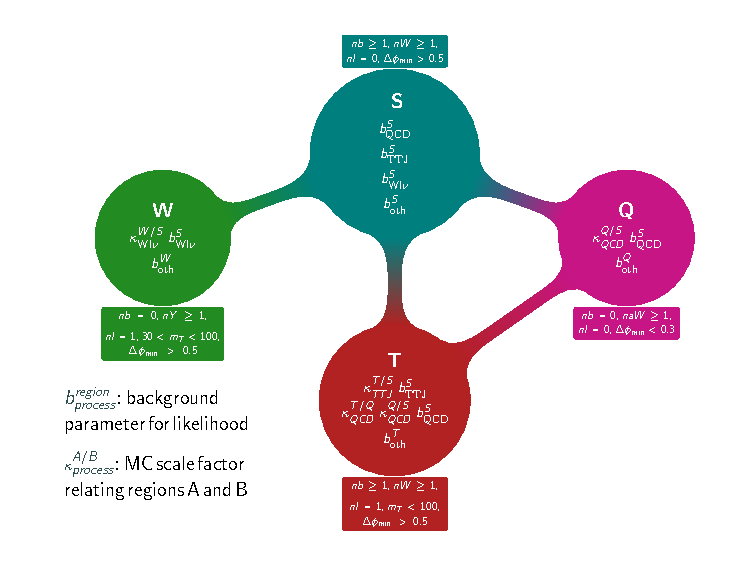
\includegraphics[width=\textwidth]{figures/BoostFlowChart_noZ}
% \caption{Definition of, and relationship between, 
% the signal ($S$) and control ($Q,T,W$) regions and their relationship
% to the bin-by-bin  background parameters $b^{region}_{process}$ for a given region and background
% process, as well as the
% four global scale factors $\kappa^{A/B}_{process} = \sum_i b^A_{process, MC, i} / \sum_i
% b^B_{process, MC, i}$, where the sum is over all bins of the simulated data. 
% The total expected background, per bin, is the sum of the terms shown for each region. Furthermore,
% associated with each bin
% of each region is an observed count, $N^{region}$, simulated count, $N^{region}_{process, MC}$, and 
% a count $N^{region}_{oth, MC}$ equal to the sum of the smaller backgrounds, with associated
% parameter $b^{region}_{oth}$.
% \label{fig:BoostWorkflow}}
% \end{figure}

The baseline selection for the Razor Boost analysis is driven by the two components of its name, in
addition to requiring the event to be of good quality.
As we use the razor variables, we need to be able to compute them. This means that there should be
at least two jets in the final state. The megajets from which the razor variables are computed, are
constructed from the AK5 jets.  
After sensitivity studies, it was decided to raise the requirement on the jet multiplicity from two
to three, reducing the background, while maintaining very good signal efficiency. The signal
processes that are the main focus of this analysis usually have even more reconstructed jets. In
order to remain as inclusive as possible, we did not, however, raise this threshold further.
%Figure~\ref{fig:njets_sig_BG} shows the distribution of the number of jets in the signal region. 
The minimal requirements on the razor variables themselves are $\mr > 800\GeV$ and $\rsq > 0.08$.
This selection is complementary to that of previous razor analyses. By requiring a larger
minimal \mr, consistent with the boosted scenario, we can explore the low \rsq region, which is
important for signals with more compressed mass spectra.
Access to the boosted phase space is also provided by making the requirement that at least one AK5
jet satisfies $\pt > 200\GeV$. 

In summary, events are required to satisfy the following baseline selection:
\begin{enumerate}
 \item Satisfy all cleanup filters, as listed in Section~\ref{event_cleaning}
 \item Have at least one good primary vertex
 \item Have at least three selected AK5 jets of which at least one has  $\pt > 200$\GeV, thereby
 defining the boosted phase space
 \item $\mr > 800\GeV$ and $\rsq > 0.08$ (where the megajets are constructed from the selected AK5
jets)
\end{enumerate}
In addition to these requirements, we also impose the trigger conditions. 
For data events, we require that one of the triggers listed in table~\ref{tab:boost_triggers} was
fired. 
For simulated events, we apply an event-by-event trigger efficiency, as explained in
Section~\ref{sec:boost_data_trigger}. 


\begin{figure}[htbp]
 \centering
 \includegraphics[width=0.55\textwidth]{figures/njets_sig_BG}
 \caption{Distribution of the number of jets for total background and an example signal point
(T1ttcc, mgluino=1000GeV, mstop=325GeV, mLSP=300GeV), in the signal region. All cuts except for the
cut on the jet multiplicity were applied. The samples have been normalized to unit area.
 \label{fig:njets_sig_BG}}
\end{figure}

% The signal and control regions are defined by different requirements on the 
% multiplicity of leptons, and $\cPqb$-tagged and $\PW$-tagged jets.  Since
% missing transverse energy,  \ETm, in multijet events is largely due to jet mismeasurements, rather
% than
% the escape of weakly interacting particles,  the \ETm vector  will often be aligned with one of the
% jets.  
% Therefore, a good discriminant between multijet events and events with
% real \ETm  is $\Delta\phi_{min}$, the minimum of the angles between \VEtmiss and the transverse
% momentum of the leading three jets,
% \begin{equation}
%  \Delta\phi_{min} = \min{\Delta\phi(\VEtmiss, \pt_i)},
% \end{equation}
% where $i$ runs over the three AK5 jets. 
% In the $T$ and $W$ control regions, the transverse mass, $m_T$, computed from the lepton 
% transverse momentum and \VEtmiss, 
% \begin{equation}
%  m_T = \sqrt{2\pt^\ell\ETm ( 1 - \cos\Delta\phi )},
% \end{equation}
% with $\Delta\phi$ the difference in azimuthal angle between lepton and \VEtmiss, is also used to
% suppress multijet and possible signal contamination.  The distribution of $m_T$ exhibits a kinematic
% edge at the mass of the $\PW$ boson for $t\bar{t}$ and $\PW+$jets processes, an edge not present for
% signal events due to
% the extra contribution to the \ETm from the invisible neutralinos.  For the $T$ and $W$ regions, we
% require $m_T < 100$\GeV in order to reduce signal contamination, and for the $W$ region, we
% additionally require $m_T > 30$\GeV in order to reduce contamination from multijet events.   
% 
% The full details of the event selection are given in Table~\ref{tab:selection}.  
% Note that, to mimic the $W+$jets contamination in the $S$ region, events in the $W$ region have a
% lepton coming from the $\PW$ boson, and a mass-tagged boosted $\PW$ jet, which is a misidentified
% q/g initiated jet.
% Figure~\ref{fig:DataMC} shows the simulated distributions in the signal region for the
% $\mathrm{M_R}$ and $\mathrm{R^2}$ variables. 
% The $m_T$ distribution in the $T$ and $W$ regions prior to the $m_T$ and $\Delta\phi_{min}$
% selection is shown in Fig.~\ref{fig:mT}, while Fig.~\ref{fig:deltaphi} shows the $\Delta\phi_{min}$
% distribution in the $Q$ region. 
% Overall, there is a reasonable agreement between data and MC yields.  The mild discrepancies can be
% accommodated by the systematic uncertainties on the MC, and they will not affect our analysis.
% 
% \begin{table}[thbp]
% \centering
% \caption{Summary of selection for signal and control regions. \label{tab:selection}}
% \vspace{1ex}
% \begin{tabular}{lccccc}
% \hline \hline
% Selection & $S$ region & $S'$ region & $Q$ region & $T$ region & $W$ region \\ 
% \hline \hline
% number of $\cPqb$ jets        & ${\geq}\, 1$   & ${\geq}\, 1$   & 0        & ${\geq}\, 1$      & 0
% \\
% number of mass-tagged $\PW$'s & ${\geq}\, 1$   & ${\geq}\, 1$   & ${\geq}\, 1$ & ${\geq}\, 1$      &
% ${\geq}\, 1$ \\
% number of tagged $\PW$'s      & ${\geq}\, 1$   & ${\geq}\, 1$   & -        & ${\geq}\, 1$      & -
% \\
% number of anti-tagged $\PW$'s & -          & -          & ${\geq}\, 1$ & -             & - \\
% number of loose leptons       & 0          & 0          & 0        & 1             & 1 \\
% number isolated tracks        & 0          & 0          & 0        & -             & - \\
% $m_T$                         & -          & -          & -        & ${<}\,100$ \GeV   &
% 30--100\GeV\\
% $\Delta\phi_{min}$            & ${>}\, 0.5$    & ${<}\, 0.5$    & ${<}\, 0.3$  & ${>}\, 0.5$       &
% ${>}\, 0.5$\\
% \hline
% \end{tabular}
% \end{table}
% 
% 
% \begin{figure}[htbp]
%  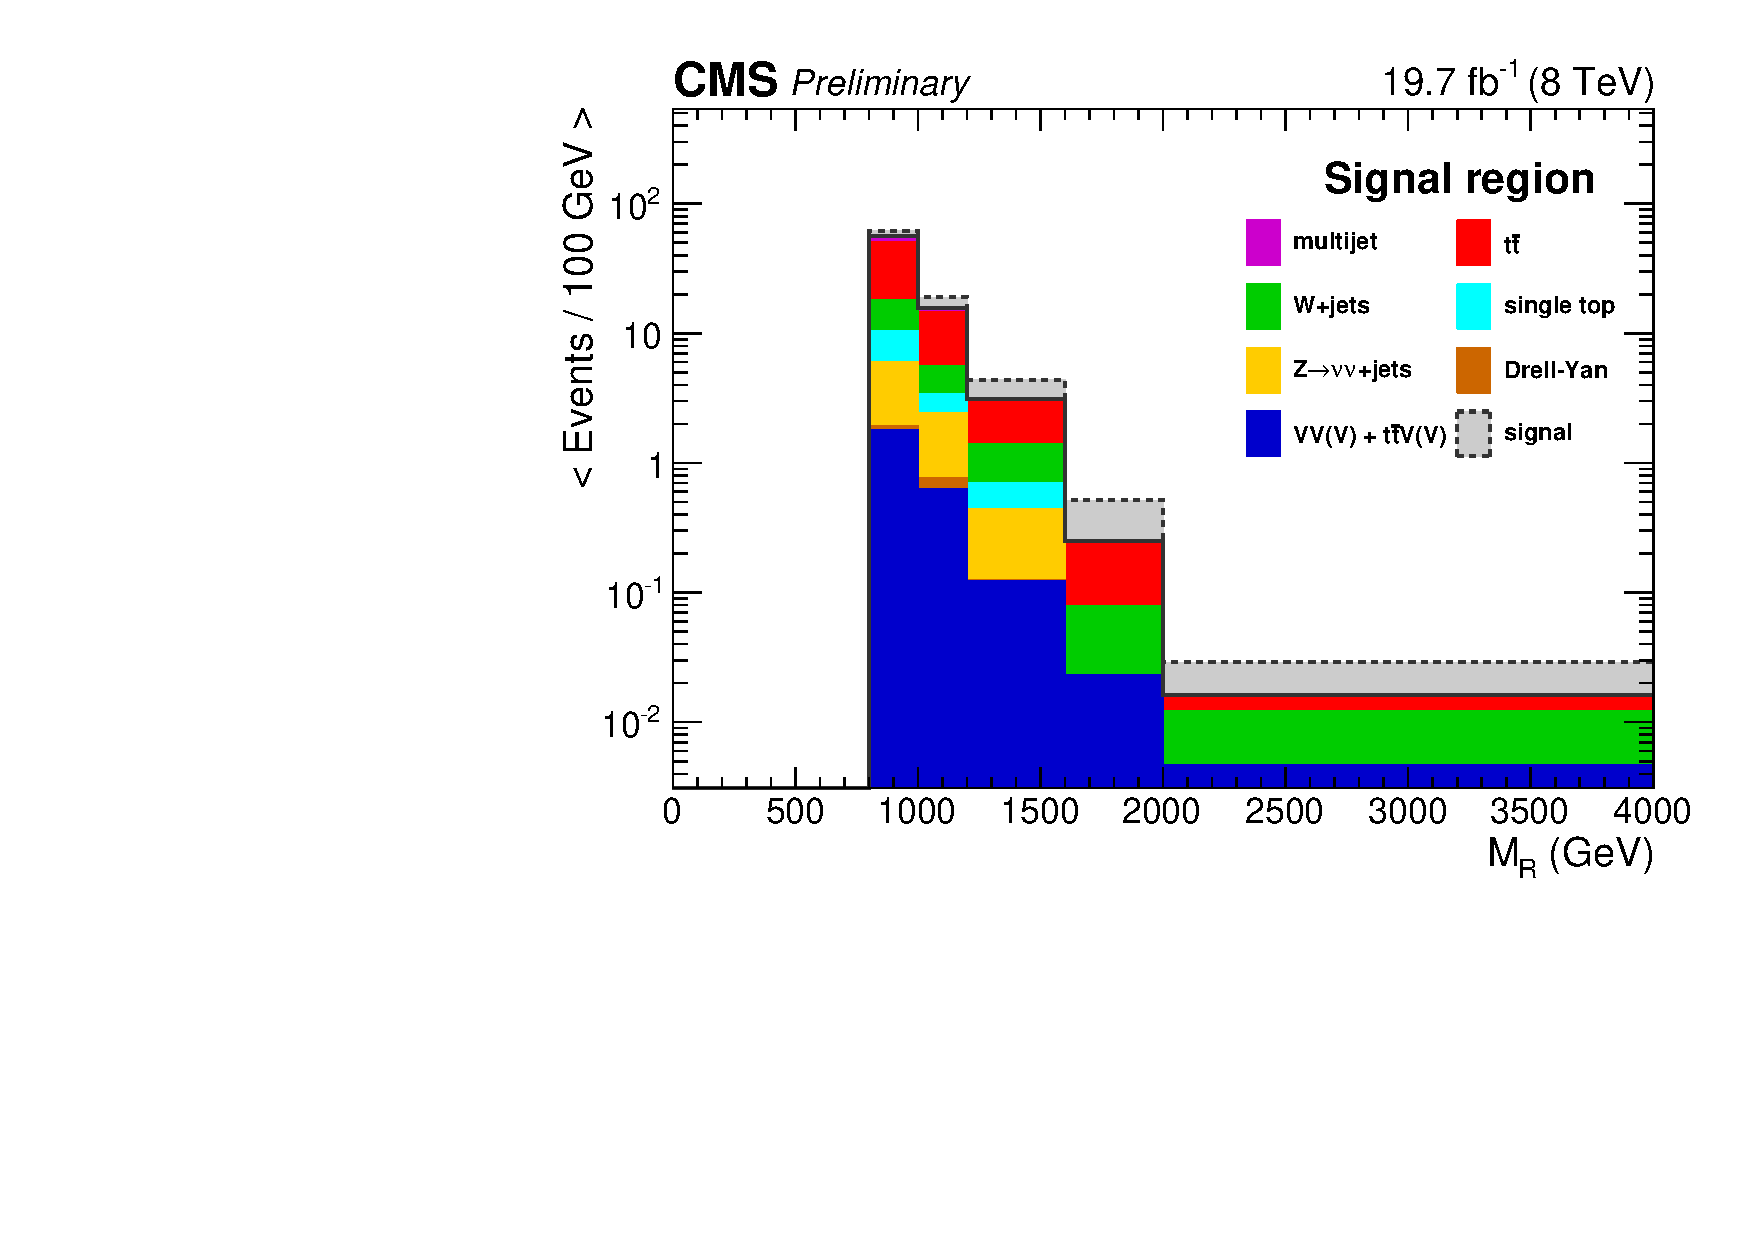
\includegraphics[width=0.49\textwidth]{figures/DataMC/DataMC_MR_g1Mbg1W0Ll_mdPhig0p5_width_nodata}
%  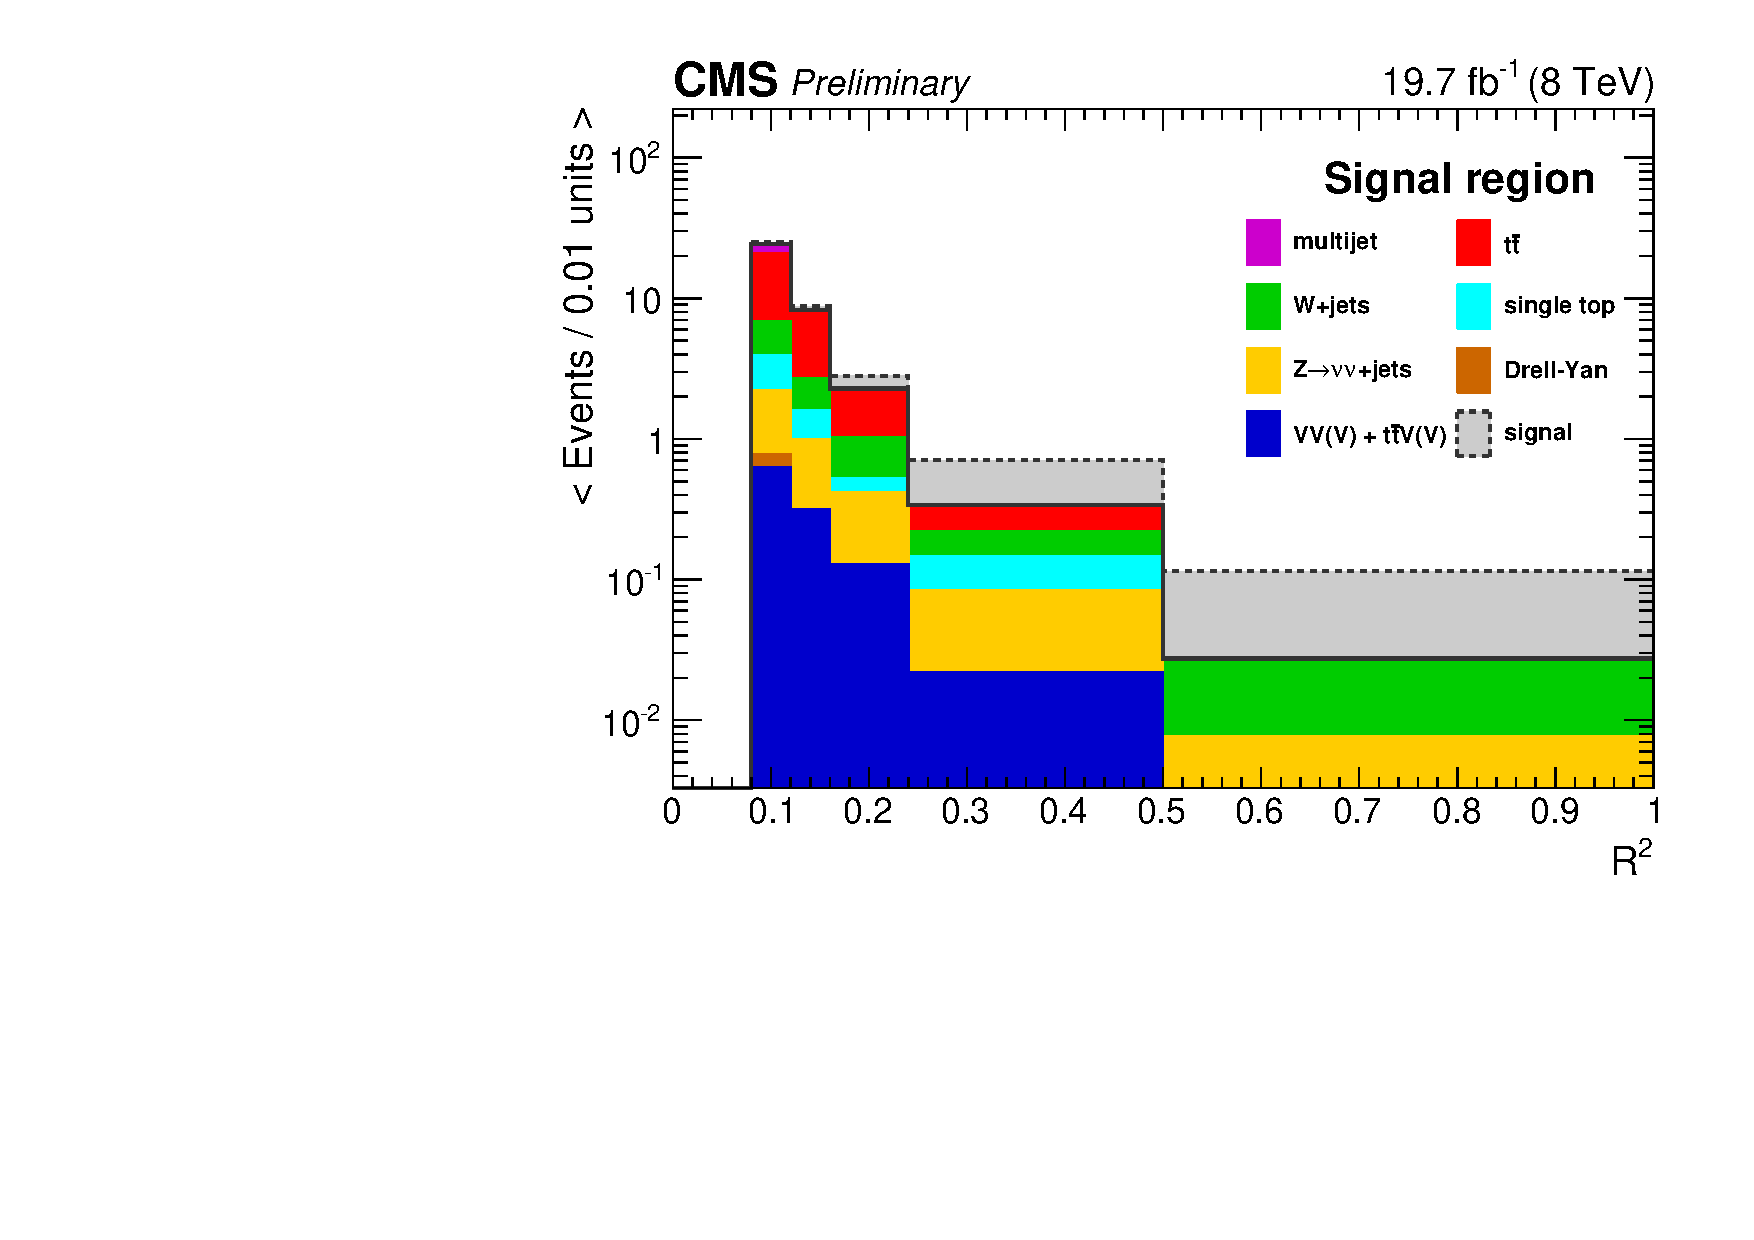
\includegraphics[width=0.49\textwidth]{figures/DataMC/DataMC_R2_g1Mbg1W0Ll_mdPhig0p5_width_nodata}
% \caption{Simulated $\mathrm{M_R}$ (left) and $\mathrm{R^2}$ (right) distributions in the signal
% region. An example signal point, corresponding to the {\it T1ttcc} mass point with $m_{\tilde{g}}
% \,{=}\, 1\TeV$, $m_{\tilde{t}} \,{=}\, 325\GeV$ and $m_{\tilde{\chi}_1^0} \,{=}\, 300\GeV$, is
% stacked on top of the background processes. The bin entries are normalized proportional to the bin
% width.  
% \label{fig:DataMC}}
% \end{figure}
% 
% \begin{figure}[htbp]
% \centering
%  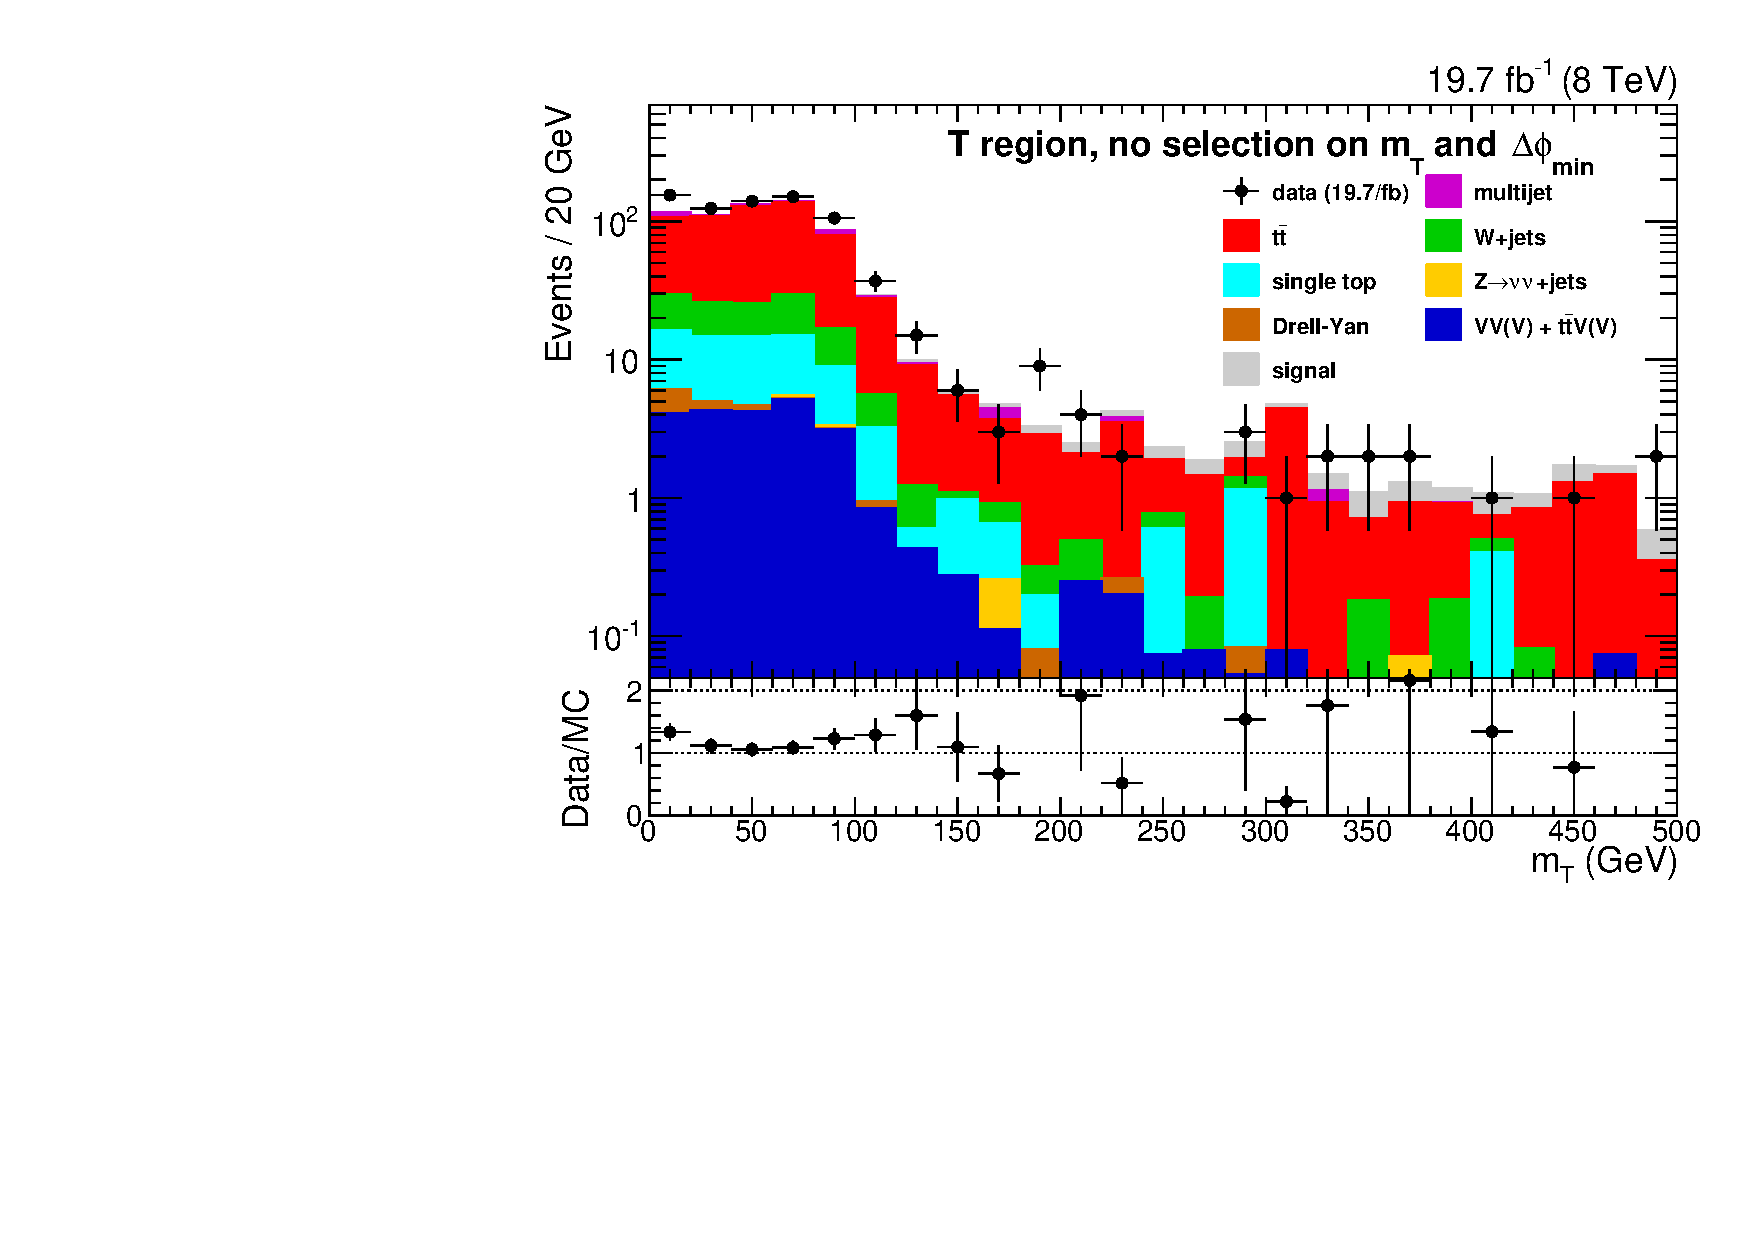
\includegraphics[width=0.49\textwidth]{figures/DataMC/DataMC_mT_g1Mbg1W1Ll_rebin}
%  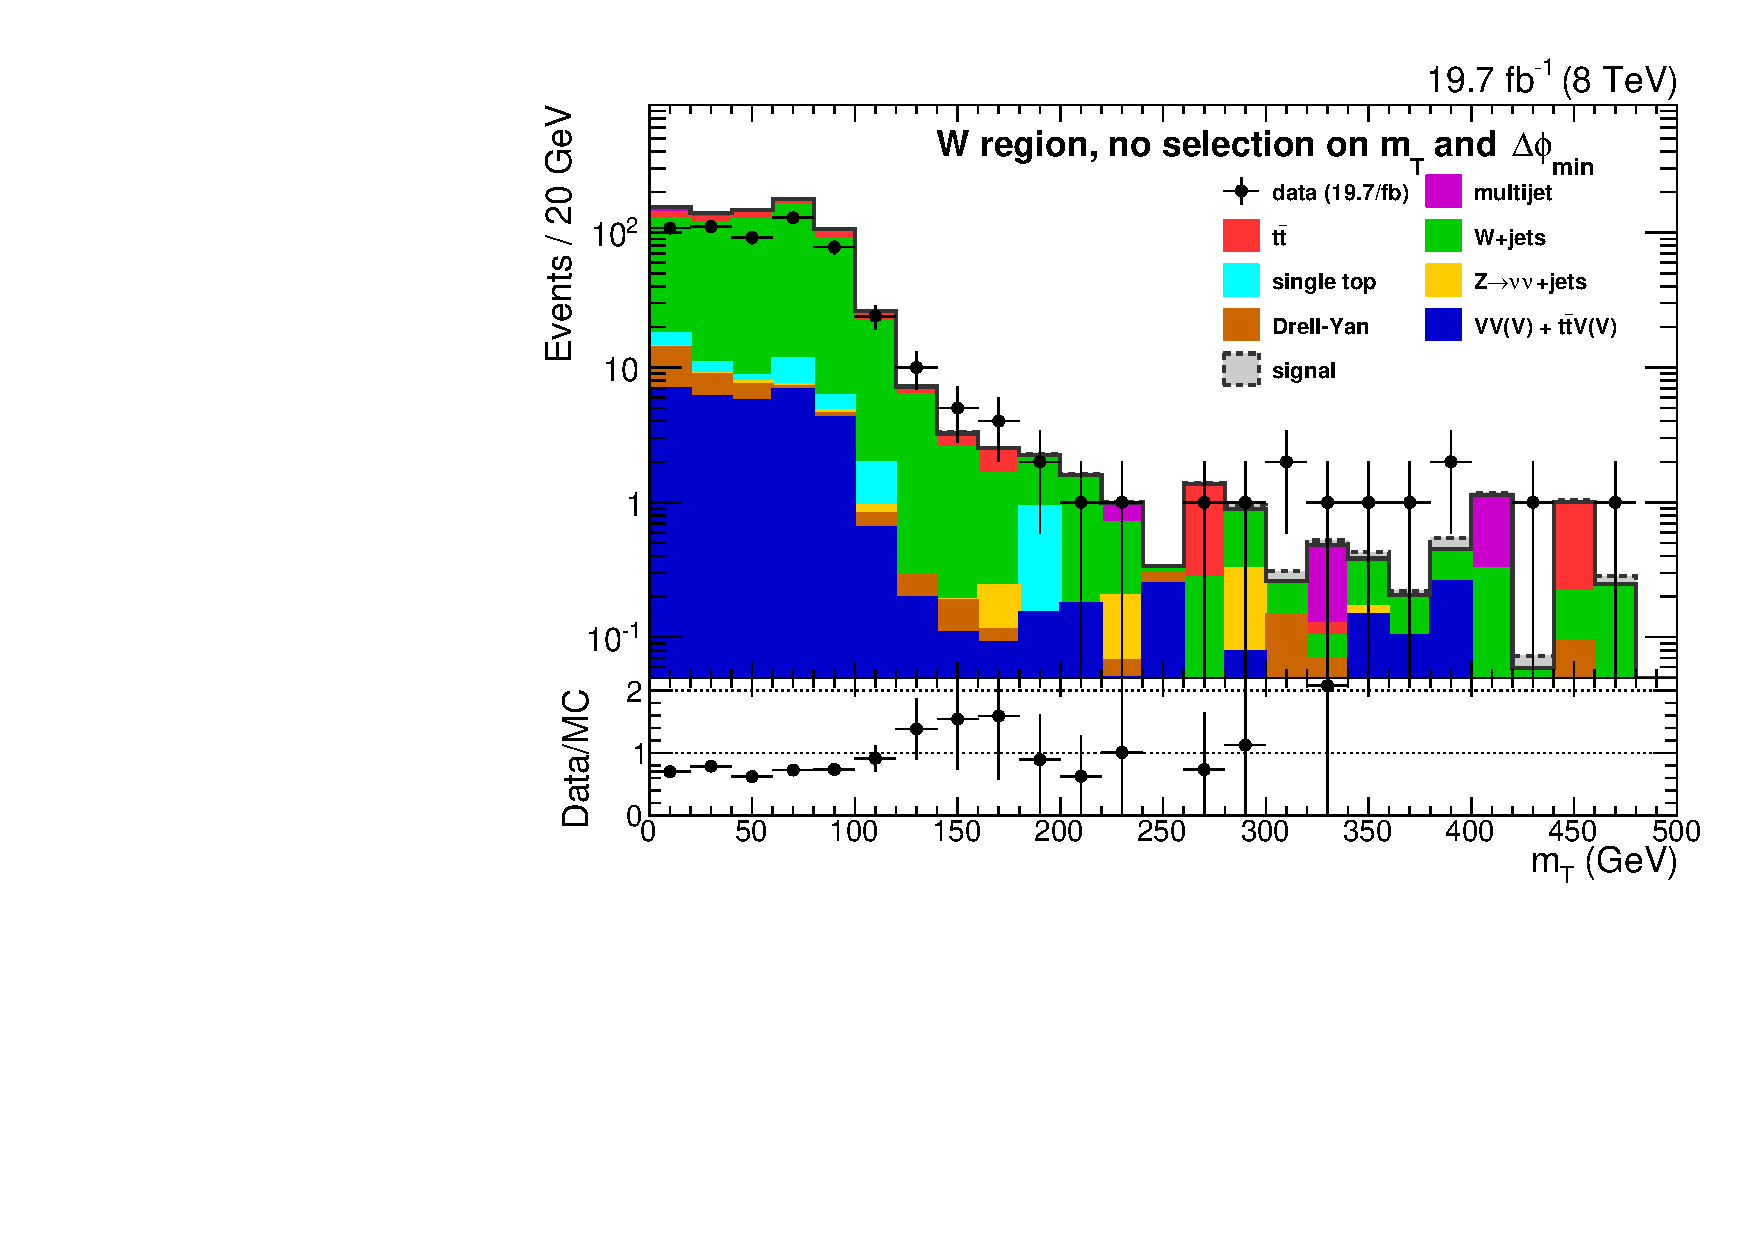
\includegraphics[width=0.49\textwidth]{figures/DataMC/DataMC_mT_0Lbg1Y1Ll_rebin}
% \caption{Comparison between data and simulation for the $m_T$ distribution in the $T$ (left) and $W$
% (right) region without applying any selection on $m_T$ and $\Delta\phi_{min}$. An example signal
% point, corresponding to the {\it T1ttcc} mass point with $m_{\tilde{g}} \,{=}\, 1\TeV$,
% $m_{\tilde{t}} \,{=}\, 325\GeV$ and $m_{\tilde{\chi}_1^0} \,{=}\, 300\GeV$, is stacked on top of the
% background processes.
% \label{fig:mT}}
% \end{figure}
% 
% \begin{figure}[htbp]
% \centering
%  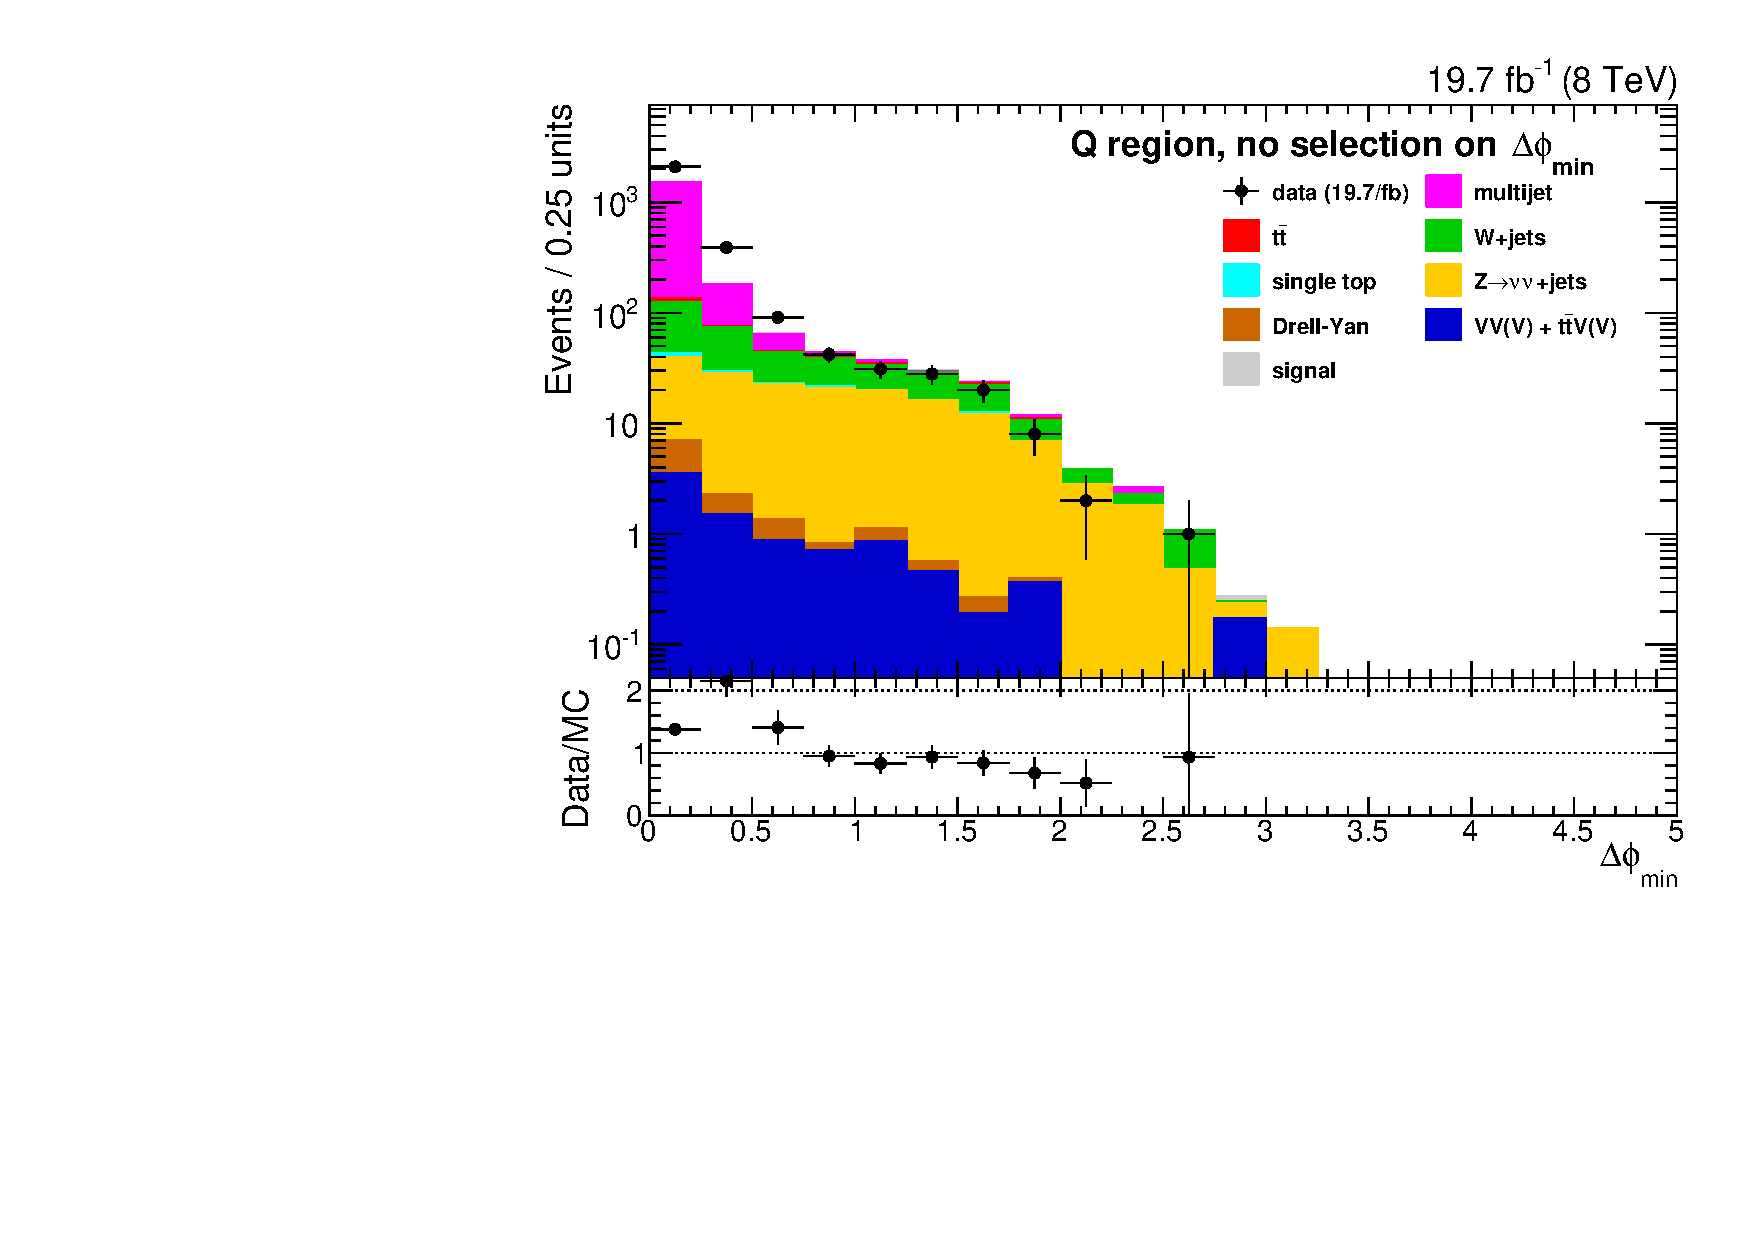
\includegraphics[width=0.49\textwidth]{figures/DataMC/DataMC_minDeltaPhi_0Lbg1uW0Ll_rebin}
% \caption{Comparison between data and simulation for the $\Delta\phi_{min}$ distribution in the $Q$
% region without applying a selection on $\Delta\phi_{min}$. 
% \label{fig:deltaphi}}
% \end{figure}
% 
% 
% In Table~\ref{tab:cutflow}, we show the expected number of events obtained from simulation for the
% different background processes and for an example signal point. The observed events in data for the
% selection levels after the trigger requirement are also reported. 
% The background composition in percent after the baseline, $S$, $T$, $W$ and $Q$ region selection is
% reported in Table~\ref{tab:BG_comp_percent}.  
% The signal region is $t\bar{t}$ dominated, with additional contributions from $\PW(\rightarrow
% \ell\nu)+$jets and multijet processes. The control regions have a good purity for the background
% process they target: 90\% for multijet, 85\% for $\PW(\rightarrow \ell\nu)+$jets and close to 80\%
% for $t\bar{t}$ and single top processes combined. 





% 
% 
% In the first section of table~\ref{tab:cutflow} we show the expected number of events for the
% different background processes for several steps in the baseline cutflow. 
% The background composition in percent after the full baseline selection is reported in
% table~\ref{tab:BG_comp_percent}.  
% In figure~\ref{fig:baseline_plots} we compare the data with the simulation for this region. The
% simulation is scaled to their expected number of events according to the (NN)LO cross sections. 
% Following corrections were applied to the simulation: pileup weights, trigger weights. Btag and Wtag
% scale factors are applied whenever there is specific requirement or veto on the number of b-tagged
% or W-tagged jets. In addition to these, the top \pt reweighting recipe was applied to the TTJets
% simulated sample. ISR weights are always applied for the signal simulation. 
% We see that there is good agreement for the highest $M_R$ and $R^2$ bins, i.e. when the contribution
% of QCD MC is very small. 
% For the first $M_R$ and $R^2$ bins, which are dominated by QCD, the MC underpredicts the data by
% about 50\%. 
% 
% \begin{sidewaystable}[p]
\centering
\caption{Cutflow table, event counts are normalized to $19.7\fbinv$. The signal is the
$m_{\tilde{g}}=1000\GeV$, $m_{\stopone}=325\GeV$, $m_{\lsp}=300\GeV$ point of the
T1ttcc scan. The row corresponding to ``$n_{PV} > 0$'' gives the event counts after applying the
cleaning filters, pileup reweighting, top \pt reweighting for $t\bar{t}$, ISR reweighting for
signal, and the requirement of at least one good primary vertex. The column indicating the total
number of events also includes some smaller processes that only contribute at the early stages of
the event selection. 
The cross sections used for each sample are listed in the second row.}
\vspace{1ex}
{\scriptsize
\begin{tabular}{ l | c  c  c  c  c  c  c  c  c | c  c  c }
%\begin{tabular}{ l || c  c  c  c  c  c  c  c  c | c || c || c }
%\begin{tabular}{| l || c | c | c | c | c | c | c | c | c | c || c || c || c |}
\toprule
Selection & Multijet & $t\bar{t}$ & $\W{\rightarrow}\ell\nu+$jets & Diboson & Single top &
$\cPZ{\rightarrow}\nu\nu+$jets & DY${\rightarrow}\ell\ell+$jets & Triboson & $t\bar{t}V$ & Total &
Signal & Data\\ 
 & $10.4\times 10^7$ pb & 245.8 pb & 111.5 pb & 95.4 pb & 114.9 pb & 588.3 pb & 22.6 pb & 0.69 pb &
1.88 pb & & 0.02435 pb & \\ 
 \midrule
% & 10.4e+07 pb & 245.8 pb & 111.5 pb & 95.4 pb & 114.9 pb & 588.3 pb & 22.6 pb & 0.69 pb & 1.88 pb & 121 pb & & 0.0243547 pb & \\ \hline \hline
No selection & $2.1\times 10^{11}$ & $4.9\times 10^6$ & $2.2\times 10^6$ & $1.9\times 10^6$ & $2.3\times 10^6$ & $1.2\times 10^7$ & $4.5\times 10^5$ & $1.2\times 10^4$ & $3\times 10^4$ & $2.1\times 10^{11}$ & 499 &  \\
$n_{PV} > 0$ & $1.05\times 10^{11}$ & $4.42\times 10^6$ & $2.02\times 10^6$ & $1.08\times 10^6$ & $1.72\times 10^6$ & $2.87\times 10^6$ & $3.7\times 10^5$ & $8.46\times 10^3$ & $2.6\times 10^4$ & $1.05\times 10^{11}$ & 479 & \\
$n_j \geq 3$ & $2.04\times 10^{10}$ & $4.08\times 10^6$ & $1.51\times 10^6$ & $5.19\times 10^5$ & $1.10\times 10^6$ & $6.24\times 10^5$ & $3.06\times 10^5$ & $5.64\times 10^3$ & $2.49\times 10^4$ & $2.05\times 10^{10}$ & 472 &  \\
$\pt(j_1) > 200\GeV$ & $1.82\times 10^8$ & $2.88\times 10^5$ & $4.36\times 10^5$ & $1.86\times 10^4$ & $6.08\times 10^4$ & $5.89\times 10^4$ & $6.61\times 10^4$ & 924 & $5.24\times 10^3$  & $1.82\times 10^8$ & 403 & \\
$M_R \,{>}\, 800, R^2 \,{>}\, 0.08$ & $3.47\times 10^4$ & $5.83\times 10^3$ & $1.17\times 10^4$ & 309 & 900 & $3.25\times 10^3$ & 422 & 40.2 & 183 & 57557 & 224 & \\
Trigger & $3.15\times 10^4$ & $5.12\times 10^3$ & $9.38\times 10^3$ & 249 & 786 & $2.32\times 10^3$ & 367 & 36.4 & 166 & 50164 & 216 & 67037 \\
\midrule
no lepton & $3.09\times 10^4$ & $1.87\times 10^3$ & $3.75\times 10^3$ & 96.3 & 311 & $2.30\times 10^3$ & 145 & 12.6 & 58.5 & 39666 & 142 & 56220 \\
\midrule[.02em]
$n_b \geq 1$ & $9.37\times 10^3$ & $1.51\times 10^3$ & 590 & 25.2 & 226 & 302 & 29.0 & 4.48 & 46.3 & 12187 & 119 & 18164 \\
$n_W \geq 1$ & 841 & 332 & 56.4 & 8.52 & 56.7 & 22.1 & 5.28 & 1.98 & 9.68 & 1350 & 28 & 1817  \\
S & 14.8 & 90.4 & 23.1 & 3.7 & 11.7 & 12.7 & 0.59 & 0.98 & 2.6 & 160 & 23.4 & 187 \\
\midrule[.02em]
$n_b = 0$ & $1.25\times 10^4$ & 98.3 & $1.70\times 10^3$ & 35.6 & 25.9 & $1.25\times 10^3$ & 46.5 & 4.19 & 3.56 & 15691 & 5.65 & 20667 \\
$n_{aW} \geq 1$ & 1519 & 18.7 & 204 & 8.36 & 7.40 & 158 & 5.41 & 0.751 & 0.819 & 1923 & 0.667 & 2712 \\
Q & 1447 & 10.6 & 93.1 & 3.88 & 3.94 & 38.9 & 3.68 & 0.28 & 0.52 & 1603 & 0.07 & 2240 \\
\midrule
1 lepton & 585.9 & $2.74\times 10^3$ & $5.52\times 10^3$ & 132 & 421 & 22.1 & 164 & 19.2 & 88.5 & 9699 & 65.0 & 10008 \\
\midrule[.02em]
$n_b \geq 1$ & 236.7 & $2.17\times 10^3$ & 625 & 29.9 & 301 & 4.14 & 28.7 & 5.36 & 68.3 & 3470 & 54 & 3930 \\
$n_W \geq 1$ & 24.3 & 496 & 61.6 & 10.0 & 50.9 & 0.56 & 3.57 & 2.36 & 16.0 & 666 & 12.3 & 770 \\
T & 0 & 112 & 20.2 & 2.0 & 13.3 & 0 & 0.38 & 0.50 & 3.2 & 151 & 1.2 & 153 \\
\midrule[.02em]
$n_b = 0$ & 150.5 & 153 & $2.86\times 10^3$ & 52.8 & 41.3 & 11.5 & 55.8 & 7.05 & 5.94 & 3329 & 2.54 & 3165 \\
$n_Y \geq 1$ & 30.8 & 79.1 & 605 & 33.1 & 13.8 & 2.4 & 13.1 & 4.57 & 2.61 & 786 & 1.19 & 581 \\
W & 0 & 15.5 & 127 & 3.6 & 1.6 & 0.64 & 0.59 & 0.52 & 0.29 & 150 & 0.06 & 116 \\
\bottomrule
\end{tabular}
}
\label{tab:cutflow}
\end{sidewaystable}

\begin{table}[htpb]
\centering
\caption{Background composition according to simulation
\label{tab:BG_comp_percent}}
\vspace{1ex}
{\small
\begin{tabular}{ l  c  c  c  c  c  c  c }
\toprule
Selection & Multijet & $t\bar{t}$ & $\W(\rightarrow \ell\nu)+$jets & Single top & $\cPZ(\rightarrow
\nu\bar{\nu})+$jets & Diboson & Other \\  
\midrule
Baseline & 62.8\% & 10.2\% & 18.7\% & 1.6\% & 4.6\% & 0.5\% & 1.6\% \\ 
$S$ & 9.2\% & 56.3\% & 14.4\%  & 7.3\% & 7.9\% & 2.3\% & 2.6\% \\
$Q$ & 90.2\% & 0.7\% & 5.8\%  & 0.2\% & 2.4\% & 0.2\% & 0.3\% \\
$T$ & 0.0\% & 73.9\% & 13.3\%  & 8.8\% & 0.0\% & 1.3\% & 2.7\% \\
$W$ & 0.0\% & 10.3\% & 84.8\%  & 1.1\% & 0.4\% & 2.4\% & 1.0\% \\
\bottomrule
\end{tabular}
}
\end{table}


% 
% \begin{figure}[htbp]
%  \centering
%  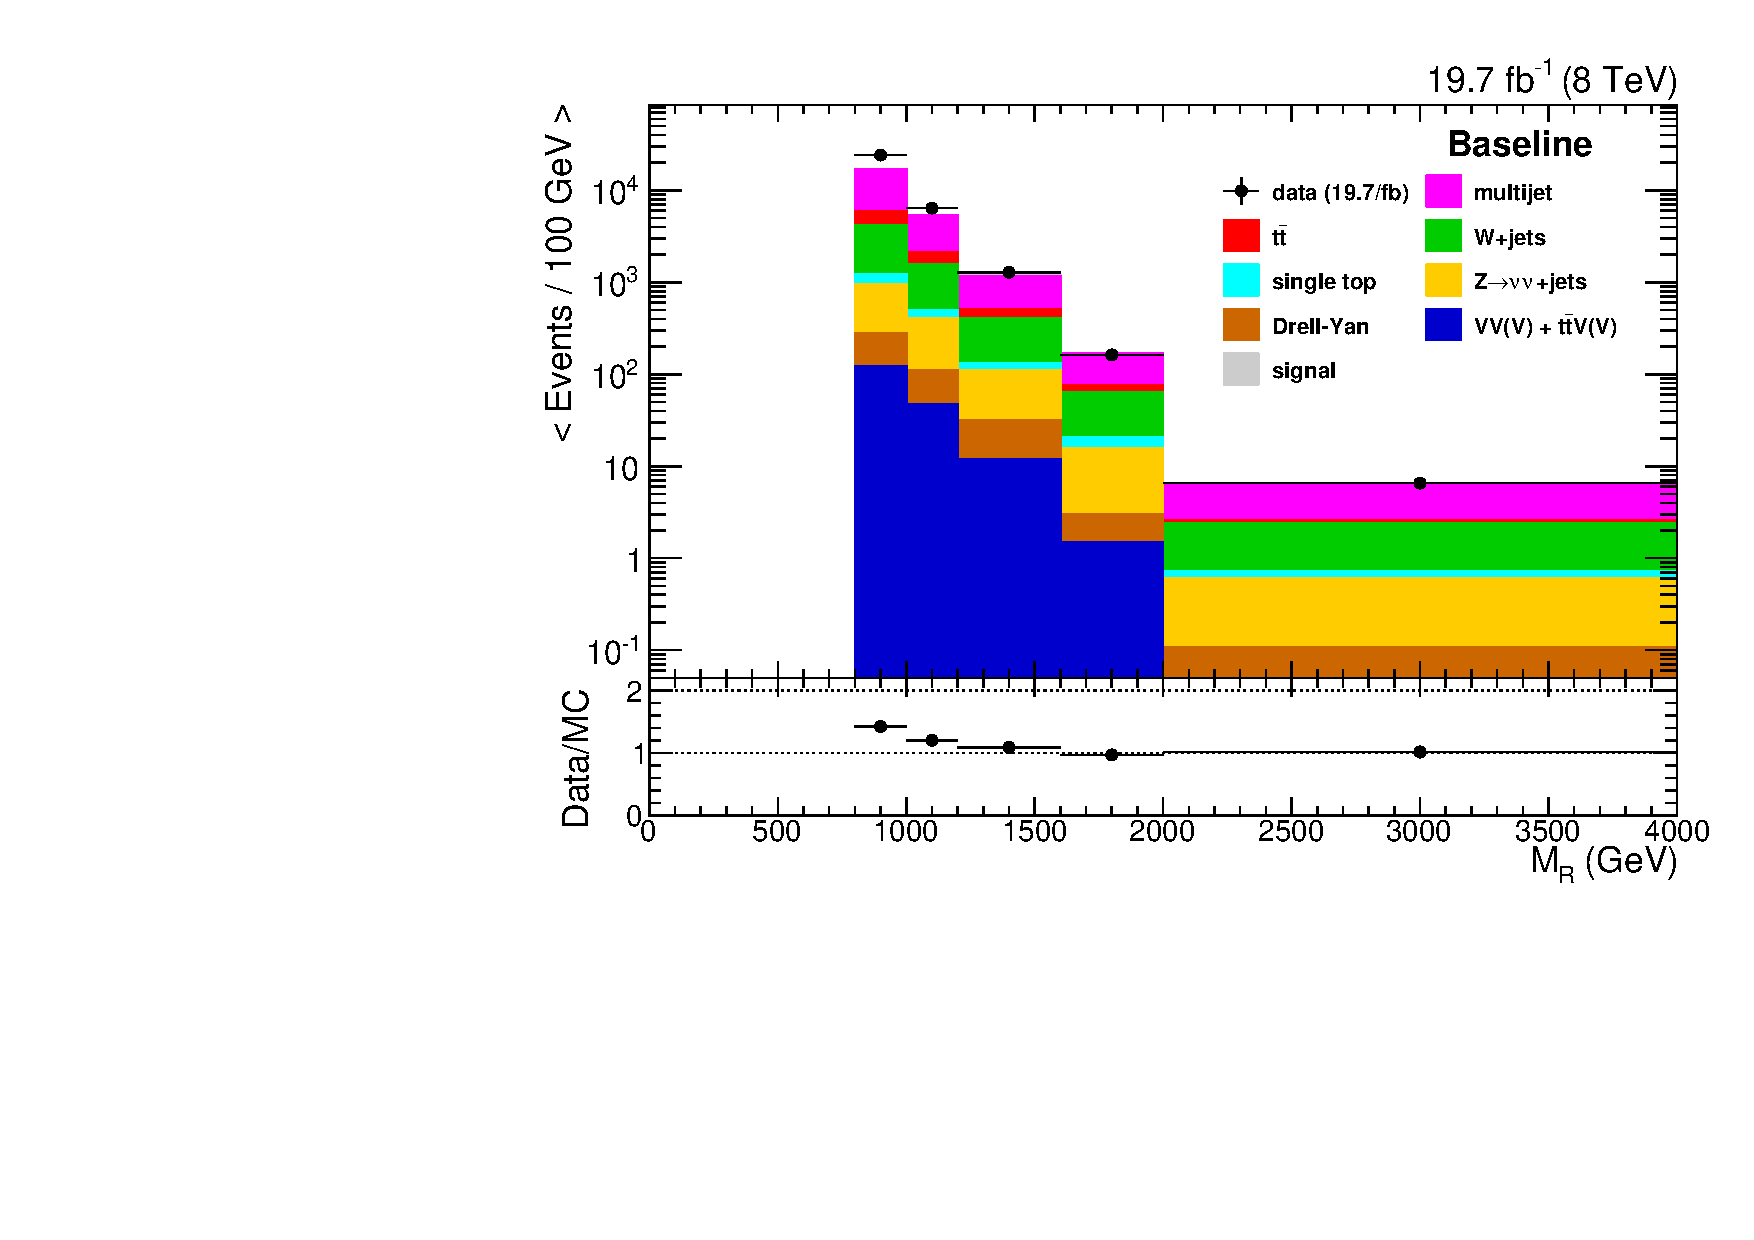
\includegraphics[width=0.49\textwidth]{figures/DataMC/DataMC_MR_HLT_width}
%  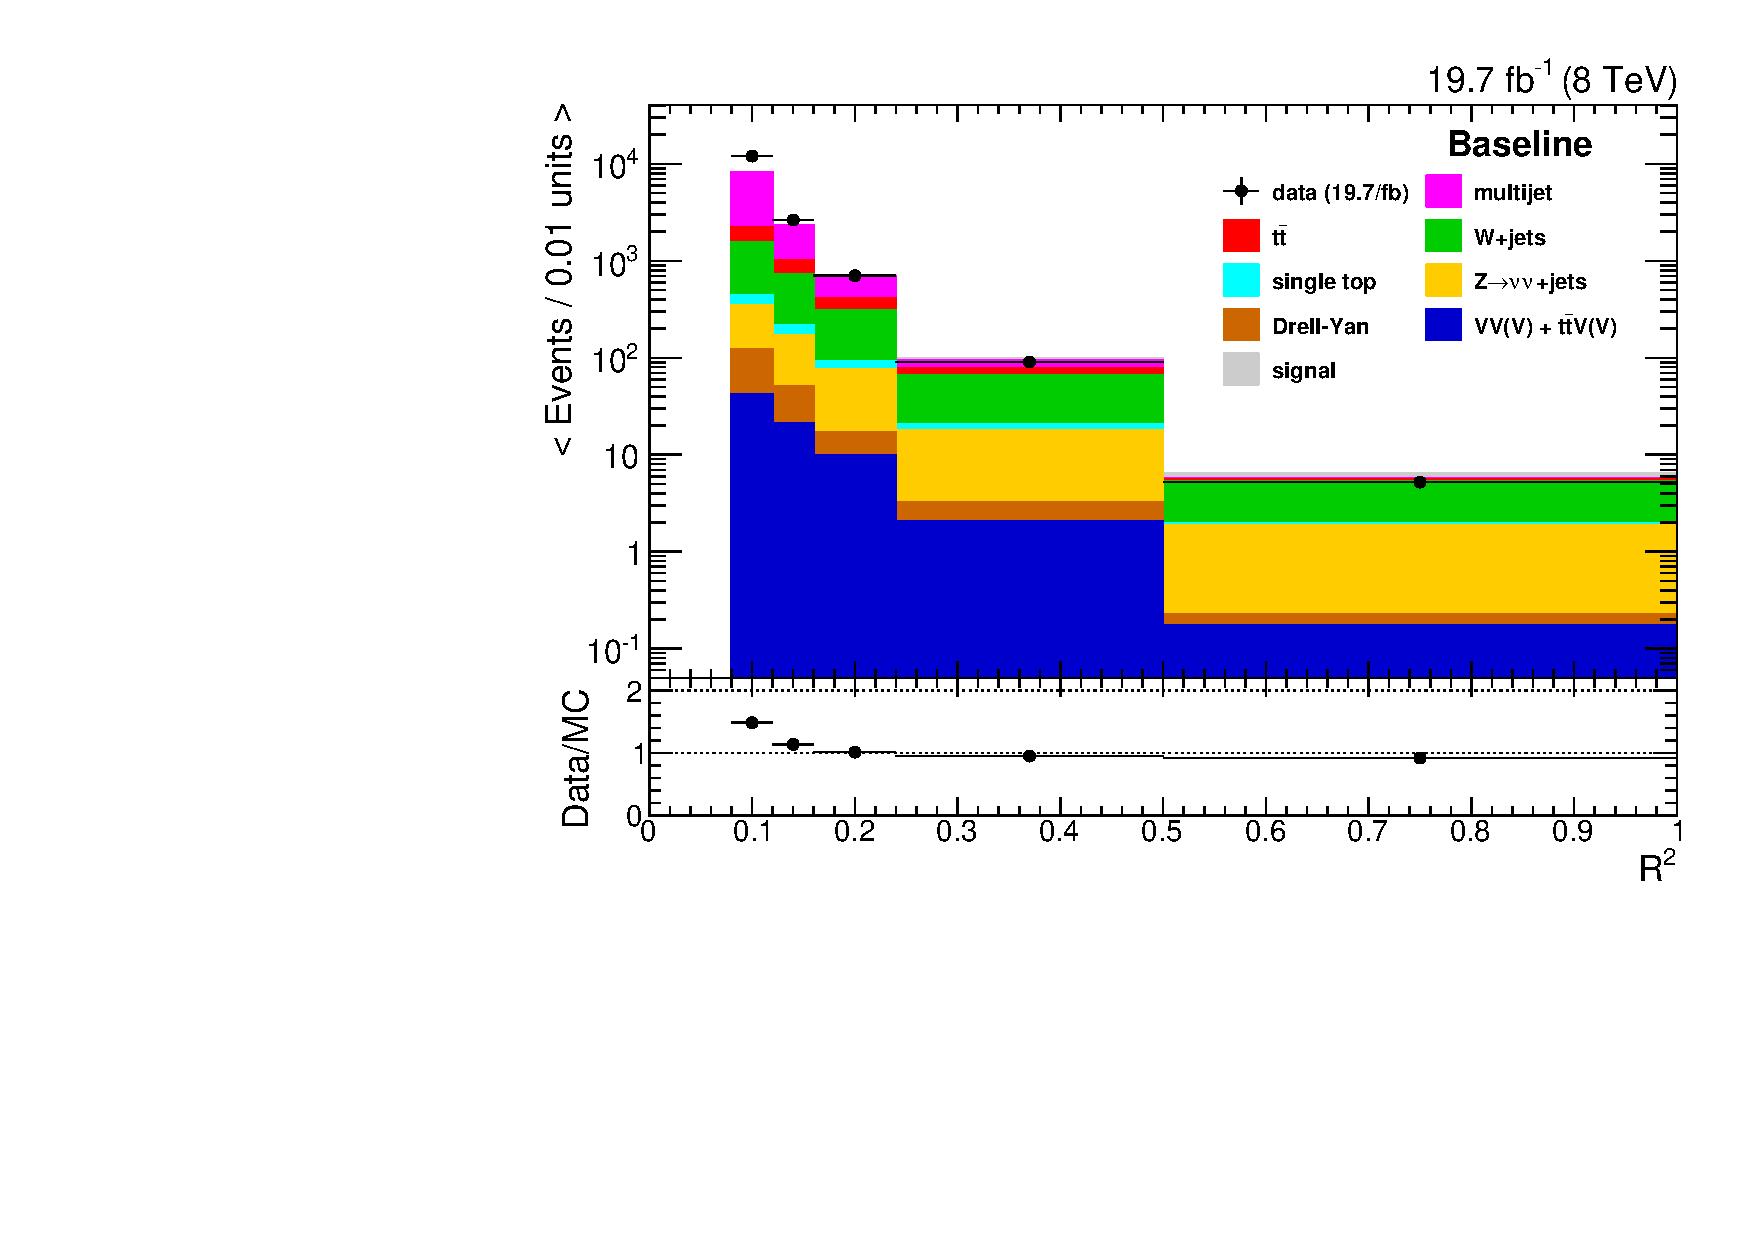
\includegraphics[width=0.49\textwidth]{figures/DataMC/DataMC_R2_HLT_width}
%  \caption{Data/MC comparison plot of $M_R$ (left) and $R^2$ (right) in the preselection region.
%  \label{fig:baseline_plots}}
% \end{figure}
